\chapter{Design} \label{chap:design}
In the previous chapter, we summarised the background for the current project, more specifically by providing a description of the technologies that we use in the design of our experiment, such as Hadoop \cite{HadoopWeb}, Global First-Fit flow scheduling \cite{al2010hedera} and fat-tree data centre topology \cite{al2008scalable}. In this chapter, the design approach and objectives of our experiment are described in Section \ref{sec:DApproach}. Subsequently, in \ref{sec:ProactiveDesign}, we describe our \textit{proactive} flow scheduling algorithm. In Section \ref{sec:DOverview}, a high level overview of our experiment design is provided and finally, in Section \ref{sec:DesignAnalysis}, an analysis of our experiment design is provided.  

\section{Approach} \label{sec:DApproach}

We propose a \textit{proactive} flow scheduling mechanism in order to determine if there are performance gains, in terms of Hadoop \cite{HadoopWeb} Job completion times and total bisection bandwidth achieved by a data centre network. 

The existing flow scheduling mechanisms described in \ref{sec:HadoopTraffic} are overwhelmingly \textit{reactive} in nature. Therefore, our approach stands as a contrast to these existing flow scheduling mechanisms, since
\begin{itemize}
	\item We configure the network before any commencement of traffic on the basis of previous executions.
	\item There is less control overhead than \textit{reactive} approaches on the network.  
\end{itemize}

Finally, by measuring our approach against existing flow scheduling mechanisms, we want to investigate if the control overhead of \textit{reactive} approaches lowers their performance.

\section{Proactive Flow Scheduling Algorithm} \label{sec:ProactiveDesign}

\begin{figure}[!ht] 
	\centerline{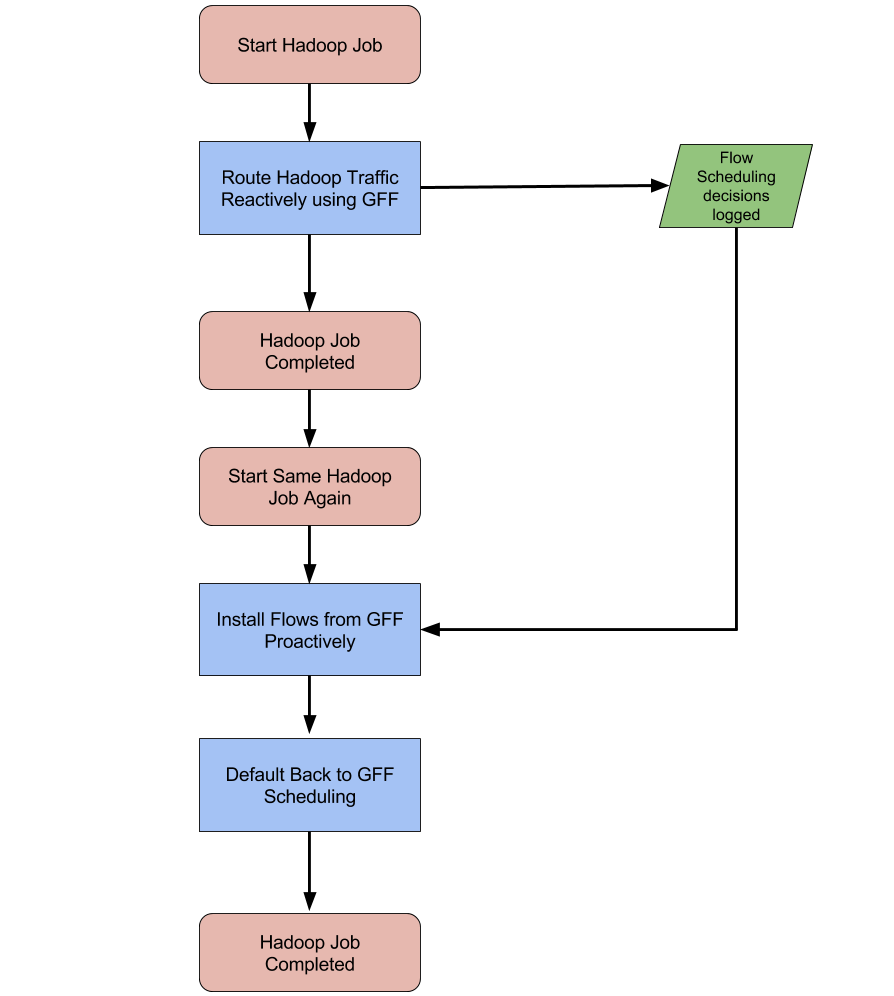
\includegraphics[scale=0.42]{graphics/chapter4/ProactiveAlgorithm.png}}
	\caption{A flowchart depicting the \textit{Proactive} Flow Scheduling Algorithm.}
	\label{fig:ProactiveAlgo}
\end{figure}
We device a proactive routing strategy as depicted in Figure \ref{fig:ProactiveAlgo} in the following steps
\begin{itemize}
	\item We run a Hadoop job on a cluster of 16 hosts, arranged in a \textit{fat-tree} \cite{al2008scalable} topology; where all switches in the network are controlled by a centralized controller using the OpenFlow \cite{mckeown2008openflow} protocol.
	\item Hadoop traffic is routed in the network using the Global First-Fit (GFF) \cite{al2010hedera} flow scheduling algorithm.
	\item The flow scheduling decisions made by the GFF algorithm are logged and persisted into the memory of the controller. 
	\item Concurrently, the total bytes transmitted and received by each host in the cluster are logged into disk, which are used to calculate the total bisection bandwidth achieved by the hosts in the network. 
	\item Subsequently, the same Hadoop Job is run again and the traffic of the network is handled by the \textit{Proactive} controller.
	\item The \textit{Proactive} controller reads the flow scheduling decisions for the same job made by the GFF algorithm earlier, and installs them statically in the network, prior to the start of Hadoop transfers.
	\item After installing flow entries statistically, it defaults to the GFF behaviour for routing flows in the network.  
	\item While the Hadoop job is running, each host in the network logs the total number of bytes transmitted and received by its network interface in order to calculate the average bisection bandwidth achieved for \textit{proactive} routing.
	\item The steps above are repeated iteratively for different Hadoop jobs. When all the iterations are completed, we obtain Hadoop Job completion times and  total bisection bandwidth utilization for our \textit{proactive} and GFF (\textit{reactive}) routing strategies.   
\end{itemize}

\section{Architecture Overview} \label{sec:DOverview}
The High-level architectural design of our experiment is illustrated in Figure \ref{fig:DesignOverview}, and it broadly consists of three parts: an SDN controller, a fat-tree data centre topology and a Hadoop Emulator. A brief overview of each part is provided in this section.
 
\begin{figure}[!ht] 
\centerline{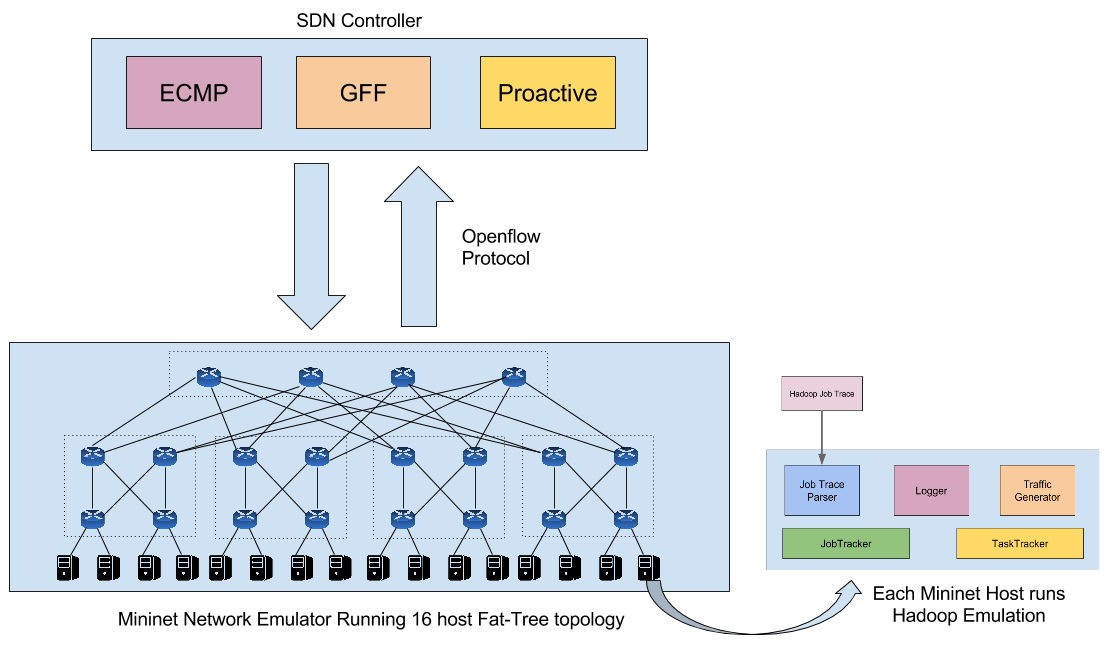
\includegraphics[scale=0.42]{graphics/chapter4/DesignOverview.png}}
\caption{High Level Overview of the experiment Design.}
\label{fig:DesignOverview}
\end{figure}

\subsection{SDN Controller}
The SDN controller has a three-fold functionality as illustrated in Figure \ref{fig:DesignOverview}. It routes Hadoop application traffic with three different routing algorithms, namely, ECMP \cite{hopps2000analysis} which is the \textit{de-facto} standard of routing traffic in a multi-rooted tree architecture \cite{al2008scalable}, Global First-Fit \cite{al2010hedera}, which is a \textit{reactive} flow scheduling algorithm that builds upon ECMP, and finally, our \textit{proactive} flow scheduling algorithm which leverages the \textit{reactive} flow decisions made by GFF for a certain Hadoop job, installing them statically before communication commences in the network for the same Hadoop job. 

At a time, it schedules flows using one of the three algorithms, which is specified when the SDN controller is launched. It controls the forwarding behaviour of all the switches in the fat-tree topology using the OpenFlow \cite{mckeown2008openflow} protocol as illustrated in Figure \ref{fig:DesignOverview}. 

\subsection{Fat-tree topology}

As mentioned in \ref{subsec:DataCentreEmulation}, we employ \textit{Mininet} \cite{lantz2010network} for emulating a data centre network, since we do not have access to a 16 host cluster. Therefore, we use the \textit{Mininet} network emulator for emulating a \textit{k}-ary fat-tree topology (described in \ref{subsec:Fat-Tree Topology}), where \textit{k} = 4 as illustrated in Figure \ref{fig:DesignOverview}. All the switches in the emulation are connected to an external SDN controller via the OpenFlow protocol, while each of the 16 hosts in the \textit{Mininet} emulator run a Hadoop emulation.

\subsection{Hadoop Emulation}

As illustrated in Figure \ref{fig:DesignOverview}, each host in the \textit{Mininet} emulator is running a Hadoop emulation. Since, the entire fat-tree topology is run on a single machine, it is not feasible to run a full version of Hadoop \cite{HadoopWeb} on the emulated hosts. Therefore, we use a lightweight alternative, by running a Hadoop emulator MRemu, on each host. As described in \ref{subsec:Mremu}, MRemu emulates Hadoop by producing iperf flows which are based on real Hadoop Job traces. Thus, we are able to simulate the running of Hadoop jobs in a 16 host fat-tree topology, where the routing decisions of the switches are controlled by an external SDN controller.   

\section{Analysis} \label{sec:DesignAnalysis}

Our aim in proposing the design of this \textit{Proactive} flow scheduling algorithm was to investigate if there are benefits in terms of better application performance and high bisection bandwidth utilization by \textit{proactive} configuration of a data centre network. 

In order to fulfil our aim, we introduced the design of our experiment in this chapter whereby we use \textit{reactive} configurations logged from the GFF algorithm, which are fed into the \textit{proactive} controller to be installed into the network as static flows. Automatic generation of proactive configuration for the network is beyond the scope of this project.

We find that the design set forth meets the requirements of this project, and is general enough to be applied to any Big data processing application traffic. It is a first step towards evaluating a \textit{proactive} measure of network configuration for big data application processing, owing to which it is straightforward to implement. The next chapter describes a proof-of-concept implementation of this design in python. 